% https://tex.stackexchange.com/questions/18292/accessing-the-logic-values-of-a-tikz-coordinate
\documentclass{article}
\usepackage{tikz}
\usetikzlibrary{calc}
\makeatletter
\def\extractcoord#1#2#3{
  \path let \p1=(#3) in \pgfextra{
    \pgfmathsetmacro#1{\x{1}/\pgf@xx}
    \pgfmathsetmacro#2{\y{1}/\pgf@yy}
    \xdef#1{#1} \xdef#2{#2}
  };
}
\makeatother
\pagestyle{empty}
\begin{document}
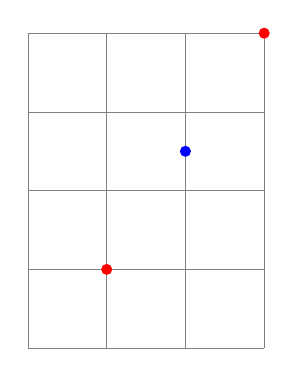
\begin{tikzpicture}
  \draw[help lines] (0,0) grid (3,4);
  \begin{scope}[shift={(1,1)}]
    \coordinate (A) at (0,0);
    \coordinate (B) at (2,3) ;
    \coordinate (C) at ($(A)!.5!(B)$);
    \fill[red] (A) circle(2pt);
    \fill[red] (B) circle(2pt);
    \fill[blue] (C) circle(2pt);
    \extractcoord\x\y{C}
  \end{scope}
  \extractcoord\xb\yb{C}
\end{tikzpicture}

Inner scope: $(\x,\y)$\par
Global scope: $(\xb,\yb)$\par
Inner scope (fixed precision):
$(\pgfmathprintnumber[precision=2]{\x},\pgfmathprintnumber[precision=2]{\y})$\par
\end{document}